% Chapter 4

\chapter{Experiments} % Main chapter title

\label{Chapter4} % For referencing the chapter elsewhere, use \ref{Chapter3} 

\lhead{Chapter 4. \emph{Experiments}} % This is for the header on each page - perhaps a shortened title

%----------------------------------------------------------------------------------------
In this chapter, experimental setup and results are described. First, the dataset is explained in detail with quantitative information. Then, feature extraction and encoding parameters and classification setups are shown and explained. Finally, results of evaluation of the proposed voting scheme are presented.
    
    \section{Experimental Setup}
    \label{section:ExperimentalSetup}
    
	    \subsection{Dataset}
        \label{section:Dataset}
        In order to evaluate the performance of the proposed voting scheme with data-driven 4D spatio-temporal patches, the dataset collected by \citet{twinanda2015data} is used. Composed of intensity and depth videos from 2 different views, the dataset has 11 days of recording of the operating room with real surgeries. The dataset is annotated with 15 different general and surgery-specific activities. The general activities are the common activities taking place in the operating room, e.g., bed entering, moving patient to OR bed, bed leaving, moving patient from OR bed, etc. The surgery-specific activities are picked from vertebroplasty procedures due to its frequency in the dataset. Vertebroplasty is a surgical procedure to stabilize the spinal fractures in which bone cement is injected through small punctures on the patient's skin to reduce pain. The dataset has 3 vertebroplasty specific activities, i.e., hammering, mixing cement and cement injection. It contains 1734 annotated video clips. Number of instances for each class are shown in Figure~\ref{fig:datasetChart}. Since the dataset is unbalanced as shown in Figure~\ref{fig:datasetChart}, bagging approach is used to balance instances from each class.


\begin{center}
\begin{figure}
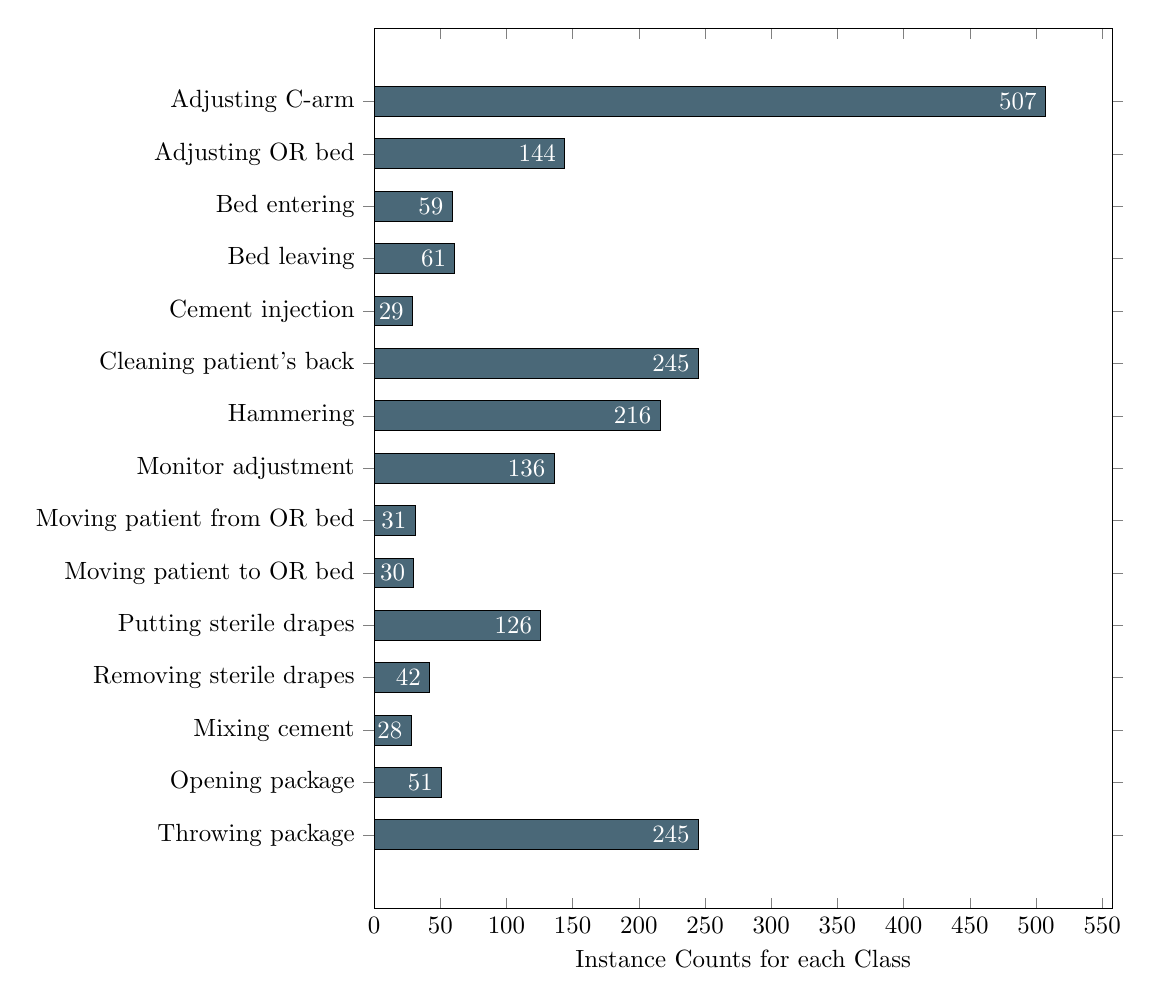
\begin{tikzpicture}[scale=0.9]
\begin{axis}[
    xbar,
    bar width=\baselineskip,
    xmin=0.0,
    width=12cm,
    height=14cm,
    ytick={1,2,3,4,5,6,7,8,9,10,11,12,13,14,15},
    yticklabels={{Throwing package},{Opening package},{Mixing cement},{Removing sterile drapes},{Putting sterile drapes},{Moving patient to OR bed},{Moving patient from OR bed},{Monitor adjustment},{Hammering},{Cleaning patient’s back},{Cement injection},{Bed leaving},{Bed entering},{Adjusting OR bed},{Adjusting C-arm}},
    enlarge y limits=0.1,
    xlabel={Instance Counts for each Class},
    ytick=data,
    nodes near coords,
    nodes near coords align=left,
    every node near coord/.style={color=white}
]
\addplot [draw=black, fill=cyan!40!black] coordinates {
    (245, 1)
    (51, 2)
    (28, 3)
    (42, 4)
    (126, 5)
    (30, 6)
    (31, 7)
    (136, 8)
    (216, 9)
    (245, 10)
    (29, 11)
    (61, 12)
    (59, 13)
    (144, 14)
    (507, 15)
};
\end{axis}
\end{tikzpicture}
\caption{Dataset Information}
\label{fig:datasetChart}
\end{figure}
\end{center}

\subsubsection{Activities in Dataset}
The dataset has 15 different activities occurs in an hybrid operating room that are shown in Figure~\ref{fig:DatasetActivities}.

\begin{itemize}
	\item \textbf{Adjusting C-Arm:} Most frequent activity in the dataset. Robotic C-Arm is moved by clinicians for taking x-ray images.
	\item \textbf{Adjusting OR Bed:} The operating room bed is moved by clinicians. 
	\item \textbf{Bed Entering:} The bed enters the operating rooms empty or with a patient.
	\item \textbf{Bed Leaving:} The bed leaves the operating room empty or with a patient.
	\item \textbf{Cement Injection:} Cement is injected to patient and during the operation operating room is dark which cause high detection in intensity data. One of the imbalance instance in dataset.
	\item \textbf{Cleaning Patient's Back:} Clinicians sterilize patient by cleaning the operation area of the patient's skin.
	\item \textbf{Hammering:} Small needle is hammered through patient's fractured vertebra with continuous x-ray captures.
	\item \textbf{Monitor or Protection Adjustment:} Clinicians adjust display monitors according to surgeons mostly before the operations. Protection equipment for x-ray beams are moved during the x-ray acquisition. 
	\item \textbf{Move Patient from OR Bed:} Patient is moved from operating room bed to portable bed after operation ends.
	\item \textbf{Move Patient to OR Bed:} After patient enters the operating room, anesthesia is applied and then the patient moved to operating room bed.
	\item \textbf{Putting Sterile Drape:} After cleaning patient's skin, sterile drapes are put to cover patient except the operating place.
	\item \textbf{Removing Sterile Drape:} After operation is ended, clinicians remove the sterile drapes and throw them to thrash.
	\item \textbf{Mixing Cement:} Cement is mixed by surgeon before cement injection procedure. Most Vertoblasty operations have one mixing cement activity. Mixing cement is the most imbalanced instance in our dataset.
	\item \textbf{Opening Package:} Packages that contain operation tools get opened on operating room tool table.
	\item \textbf{Throwing Package:} After operation ends, clinicians throw packages on the tool table to trash.
\end{itemize}

\begin{figure}[!htbp]
\centering
\subfigure[Adjusting C-Arm]{\label{sfig:a}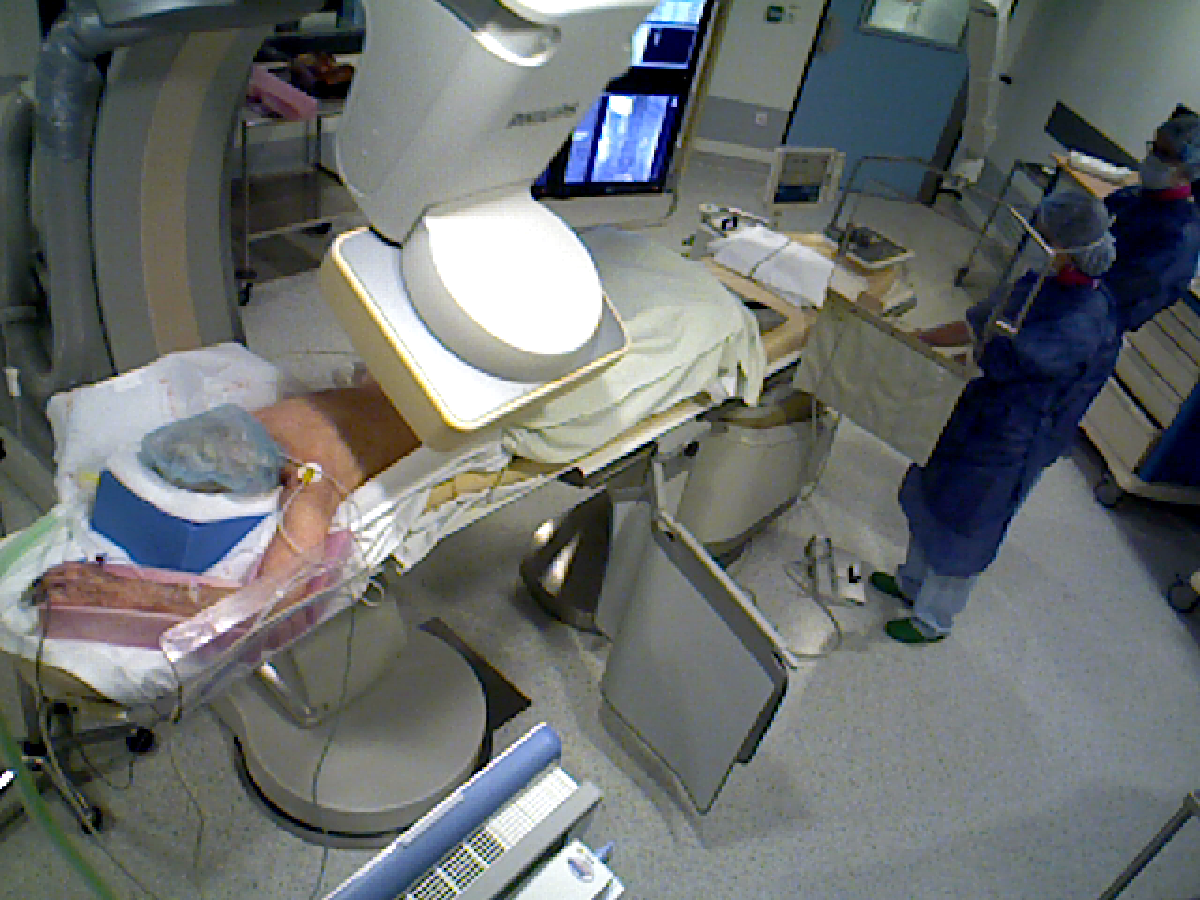
\includegraphics[width=.33\textwidth]{Figures/Actions/01_AdjustingCArm}}\hfill
\subfigure[Adjusting OR Bed]{\label{sfig:b}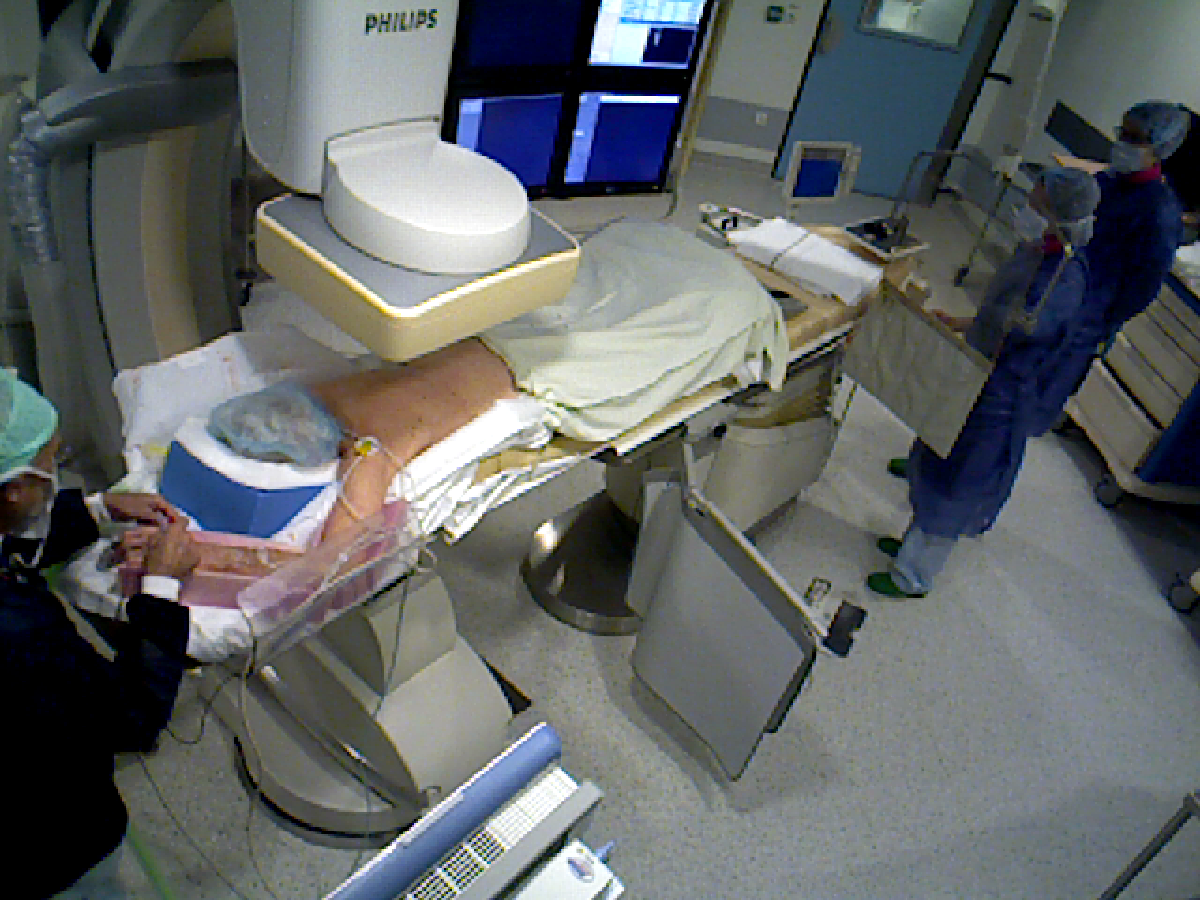
\includegraphics[width=.33\textwidth]{Figures/Actions/02_AdjustingORBed}}\hfill
\subfigure[Bed Entering] {\label{sfig:c}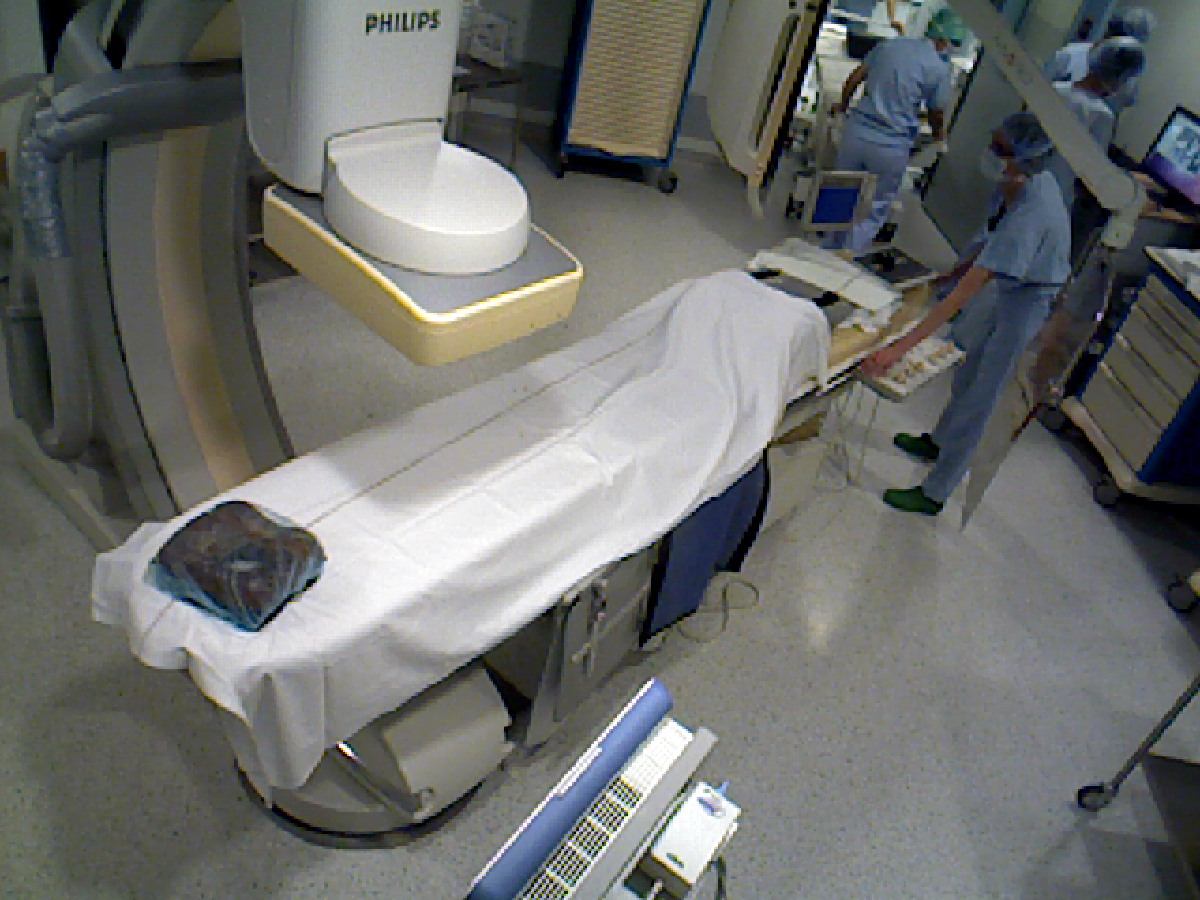
\includegraphics[width=.33\textwidth]{Figures/Actions/03_BedEntering}}\\
\subfigure[Bed Leaving]{\label{sfig:d}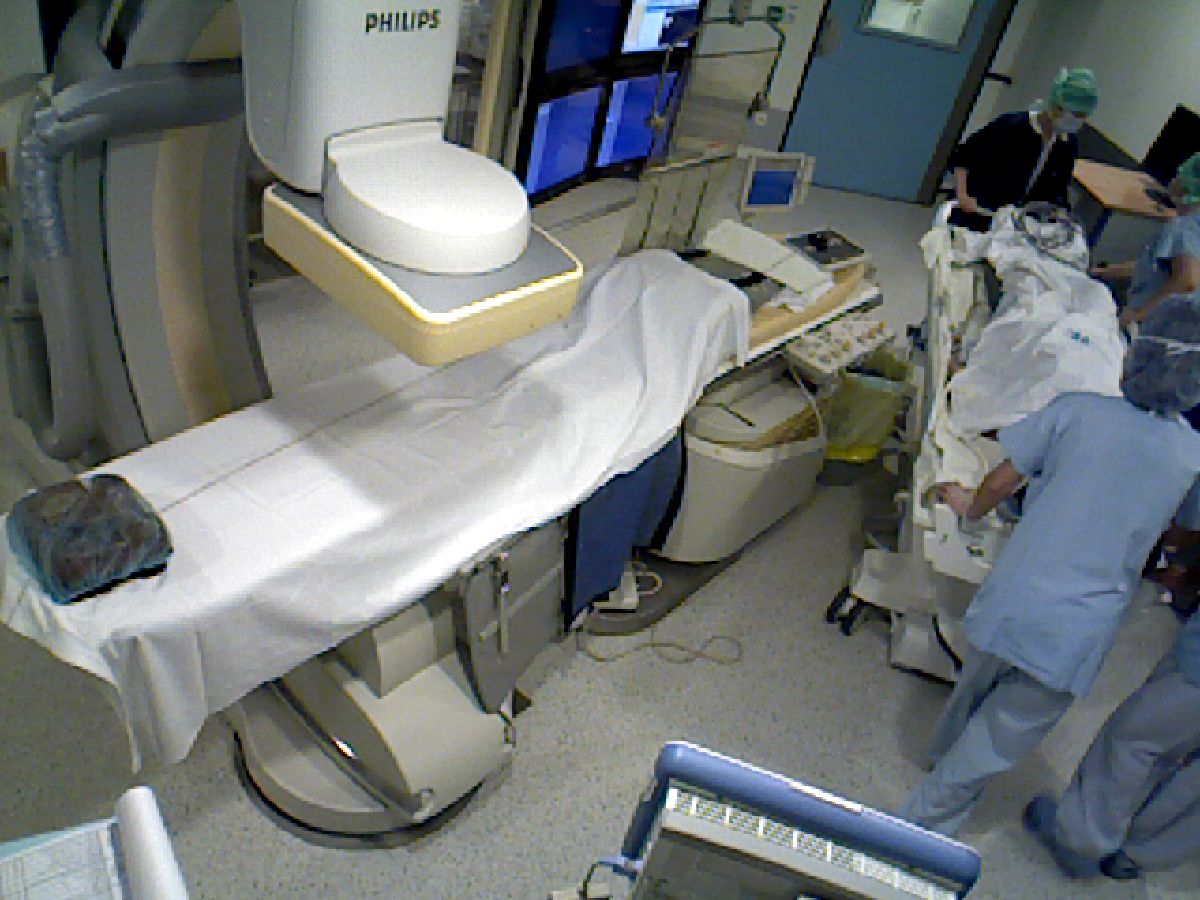
\includegraphics[width=.33\textwidth]{Figures/Actions/04_BedLeaving}}\hfill
\subfigure[Cement Injection]{\label{sfig:e}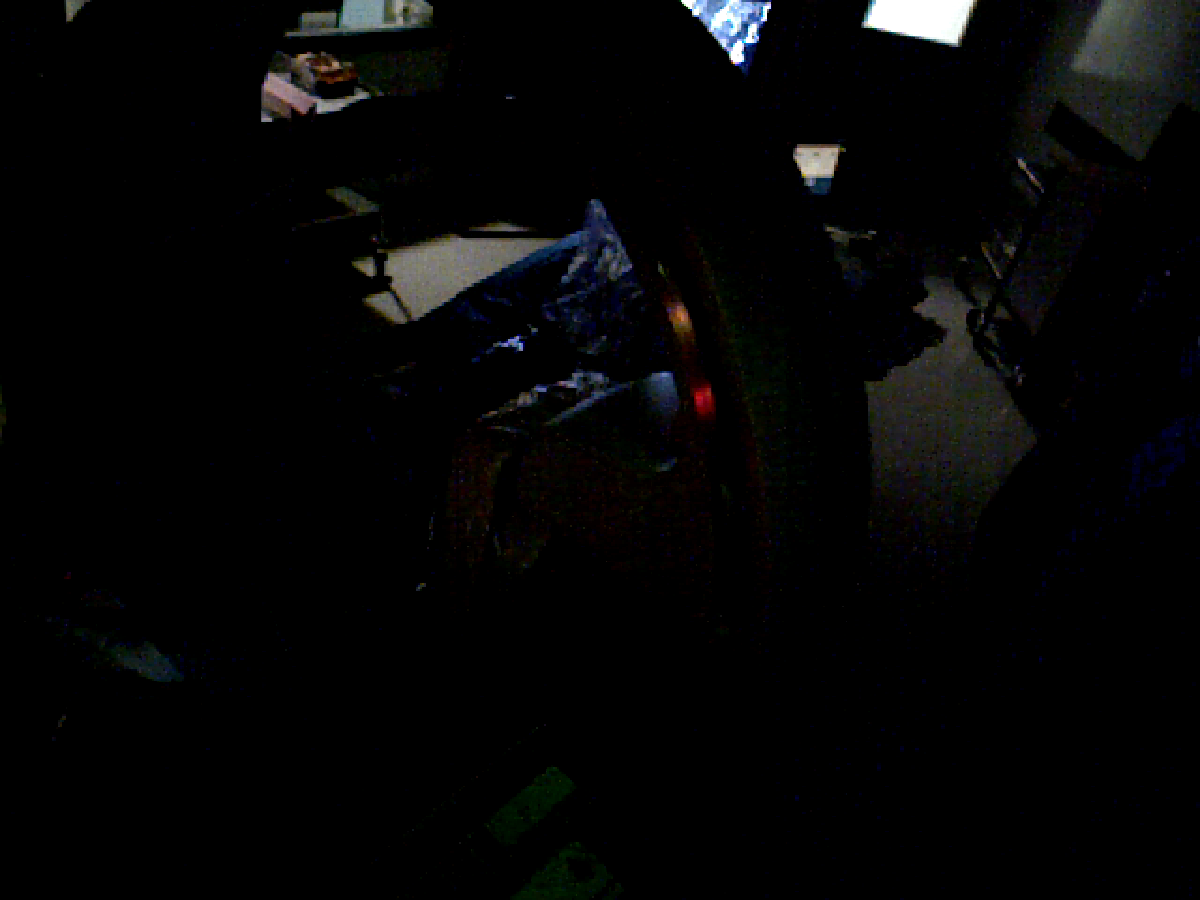
\includegraphics[width=.33\textwidth]{Figures/Actions/05_CementInjection}}\hfill
\subfigure[Cleaning Patient's Back]{\label{sfig:f}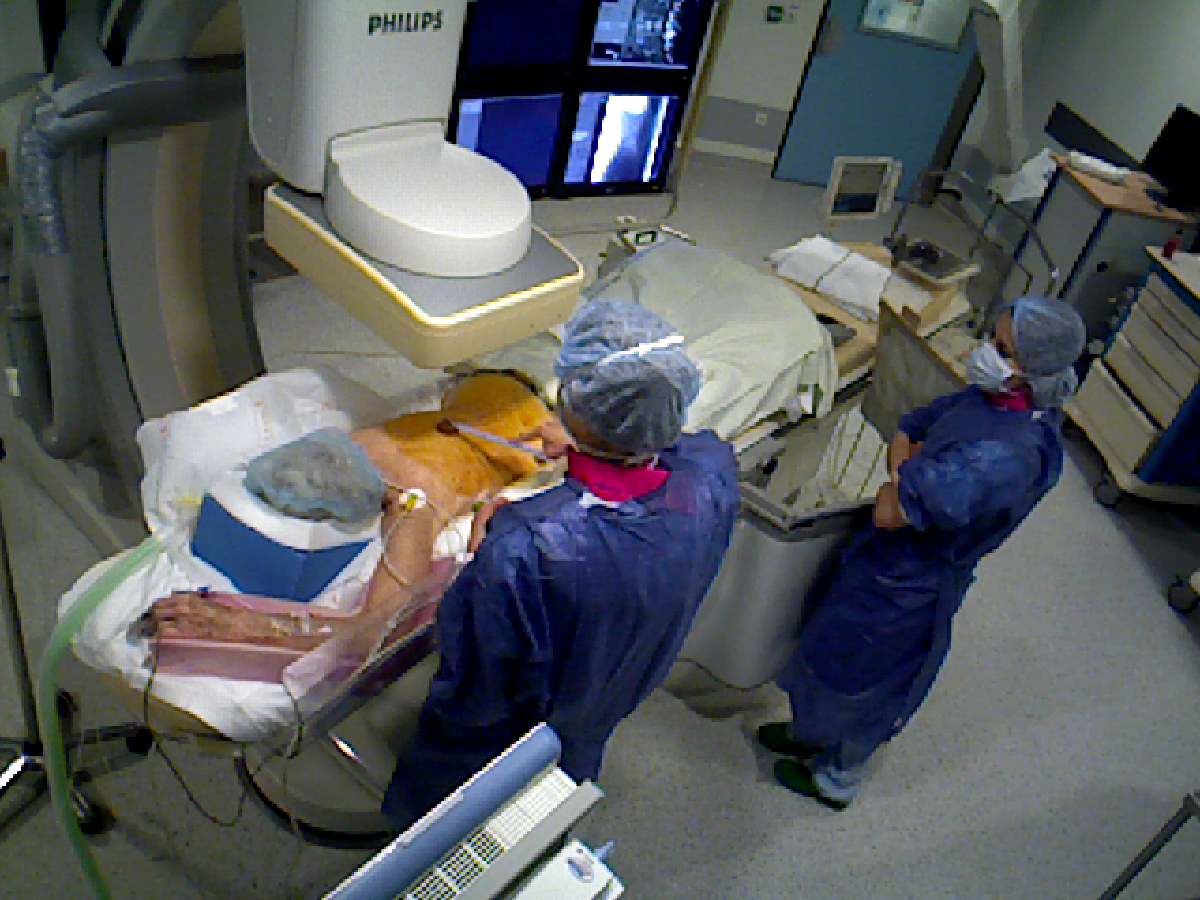
\includegraphics[width=.33\textwidth]{Figures/Actions/06_CleaningPatientBack}}\\
\subfigure[Hammering]{\label{sfig:g}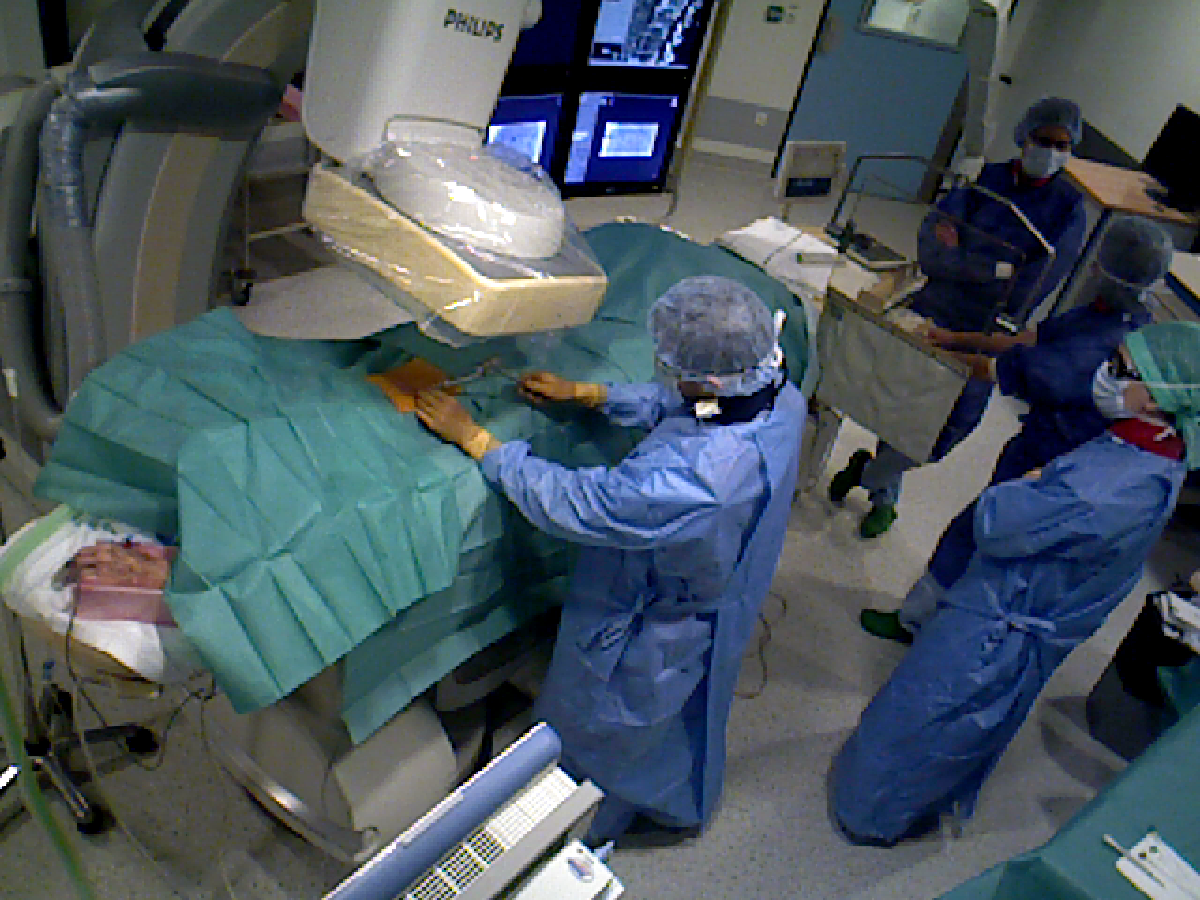
\includegraphics[width=.33\textwidth]{Figures/Actions/07_Hammering}}\hfill
\subfigure[Monitor or Protection Adjustment]{\label{sfig:h}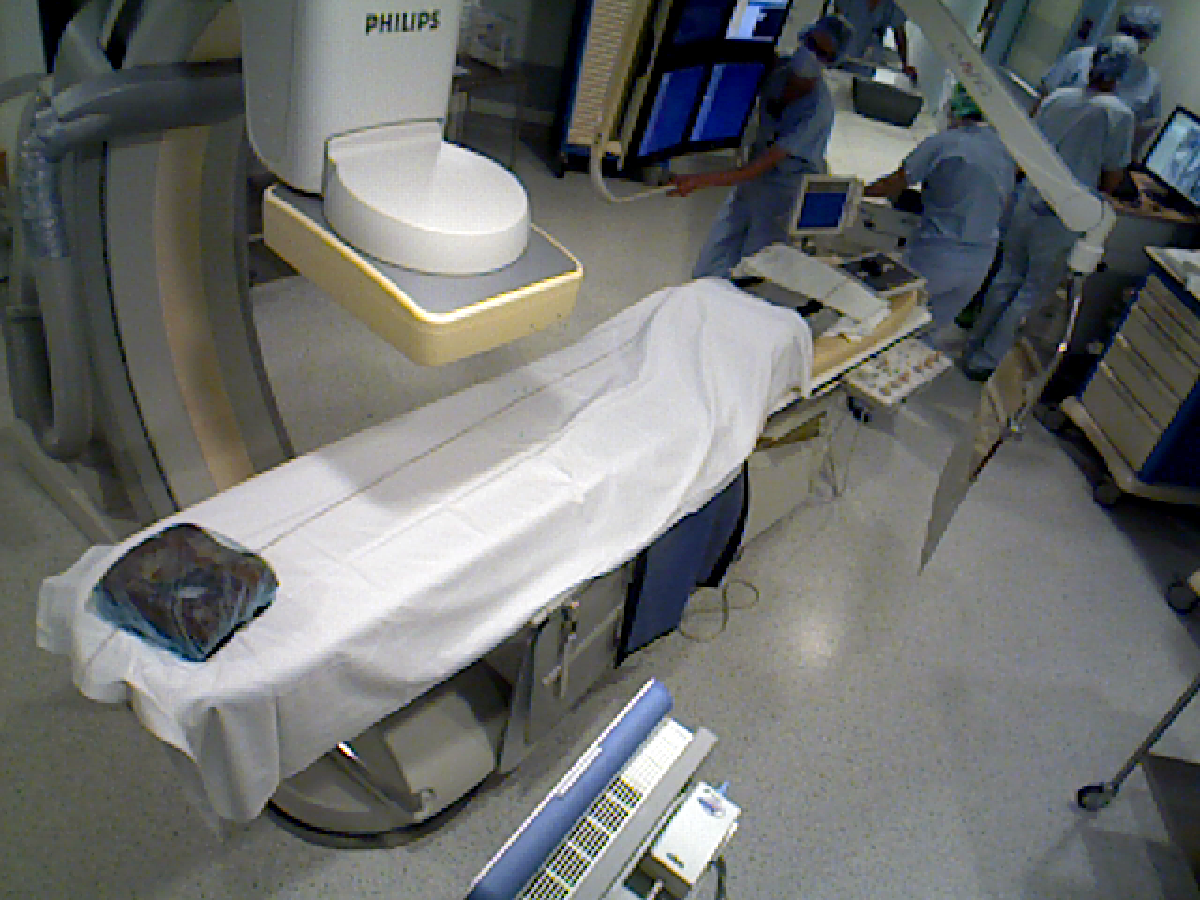
\includegraphics[width=.33\textwidth]{Figures/Actions/08_MonitorAdjustment}}\hfill
\subfigure[Move Patient from OR Bed]{\label{sfig:i}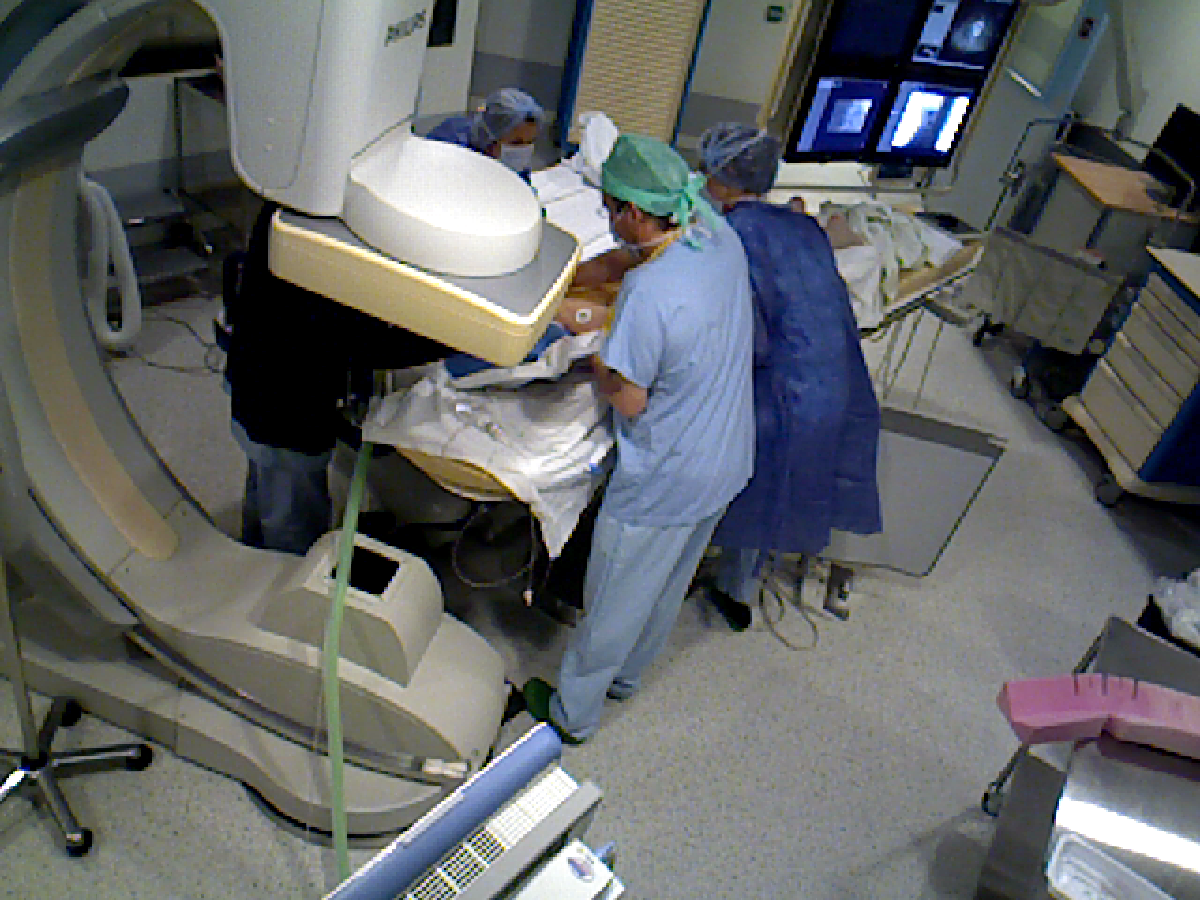
\includegraphics[width=.33\textwidth]{Figures/Actions/09_MovePatientFromORBed}}\\
\subfigure[Move Patient to OR Bed]{\label{sfig:j}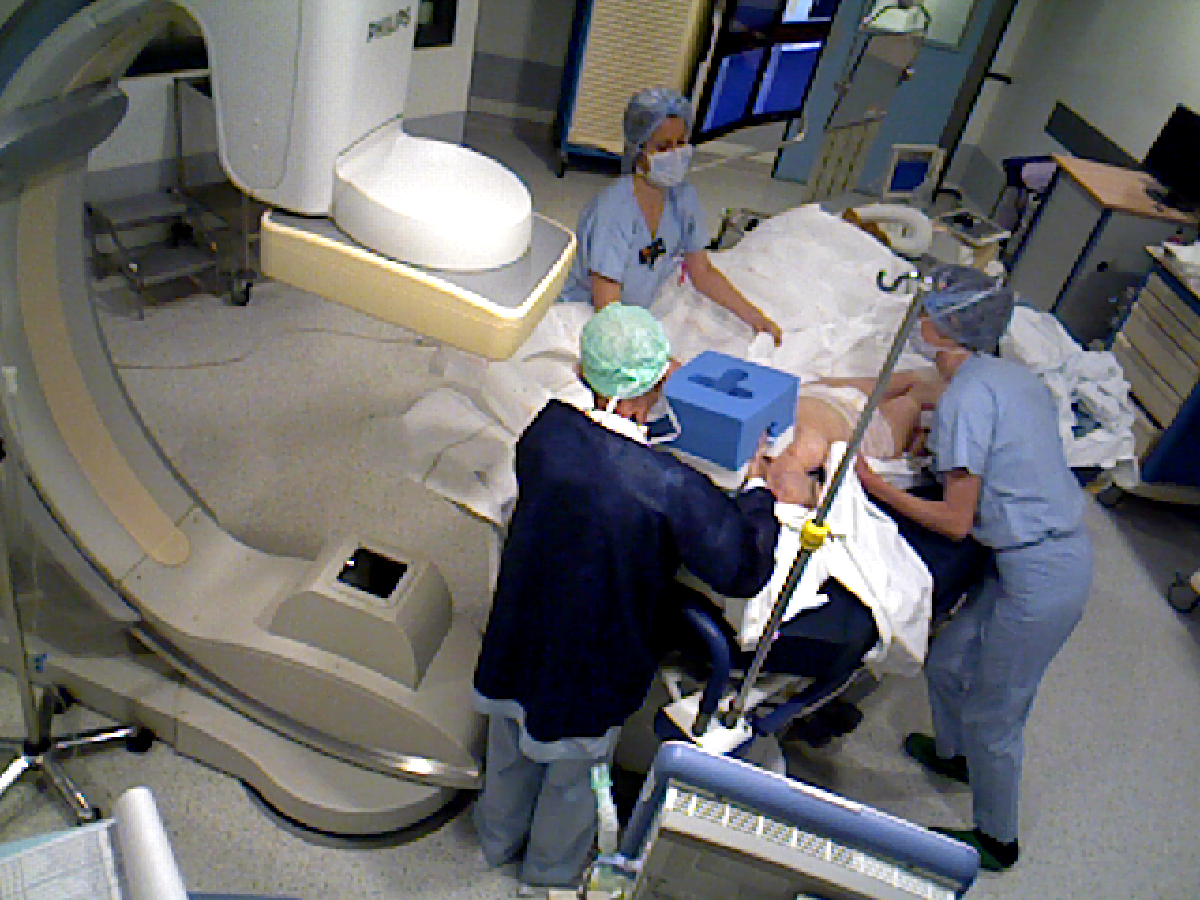
\includegraphics[width=.33\textwidth]{Figures/Actions/10_MovePatientToORBed}}\hfill
\subfigure[Putting Sterile Drape]{\label{sfig:k}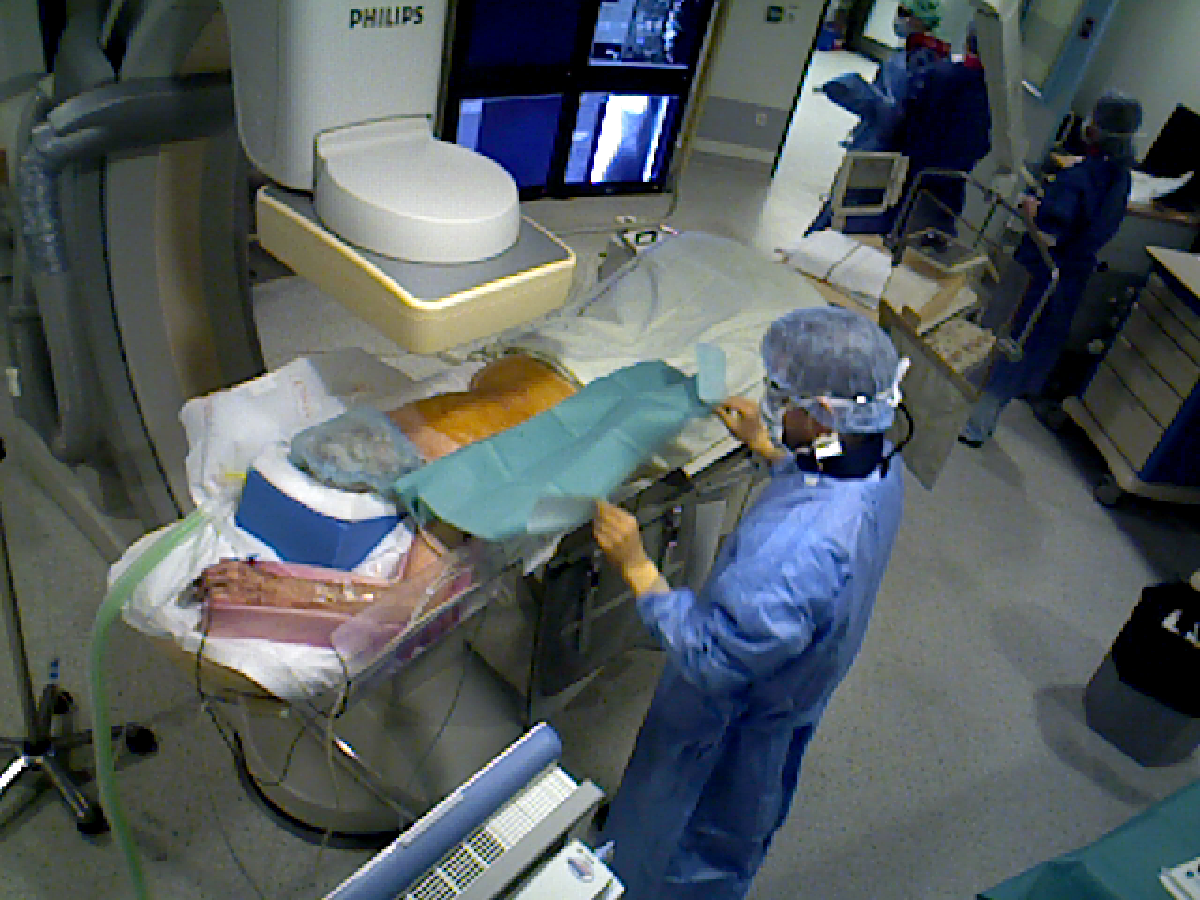
\includegraphics[width=.33\textwidth]{Figures/Actions/11_PuttingSterileDrape}}\hfill
\subfigure[Removing Sterile Drape]{\label{sfig:l}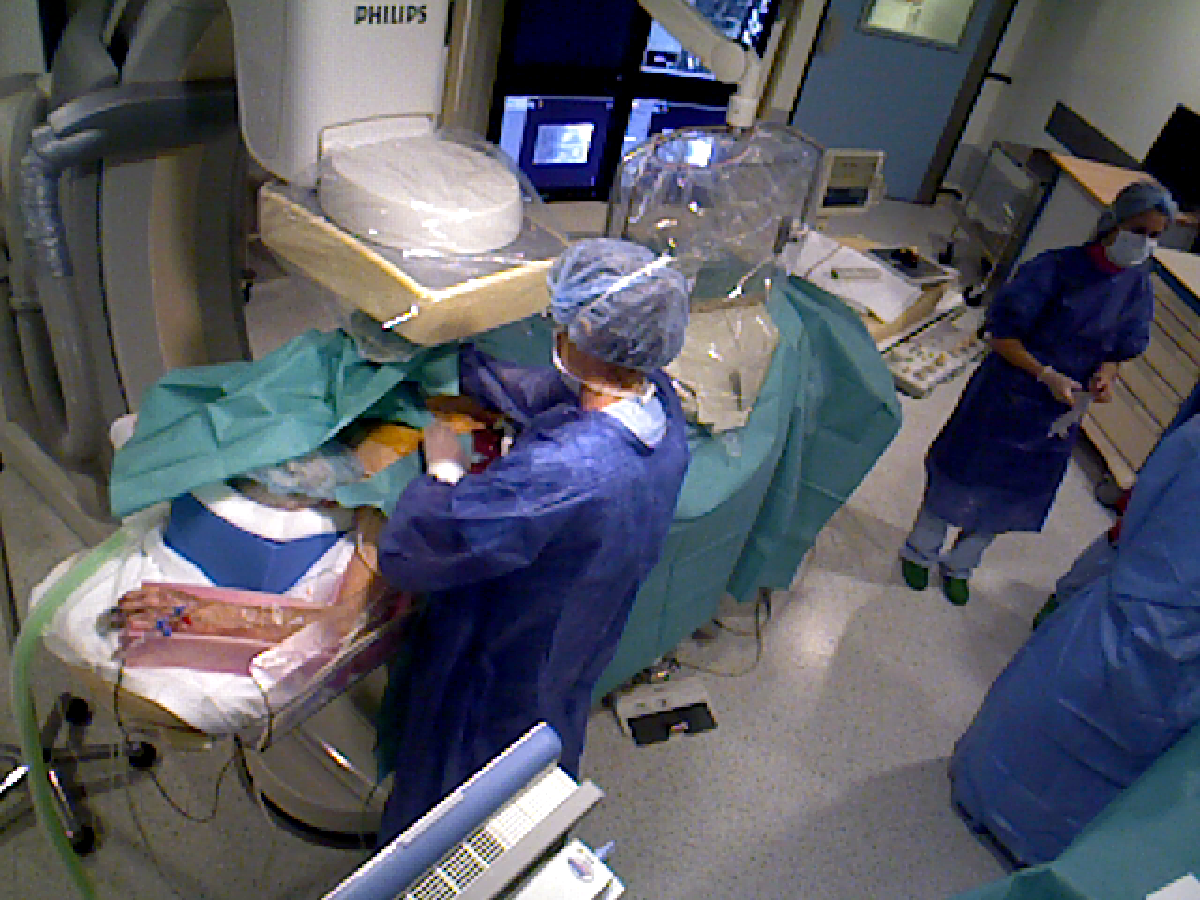
\includegraphics[width=.33\textwidth]{Figures/Actions/12_RemovingSterileDrape}}\\
\subfigure[Mixing Cement]{\label{sfig:m}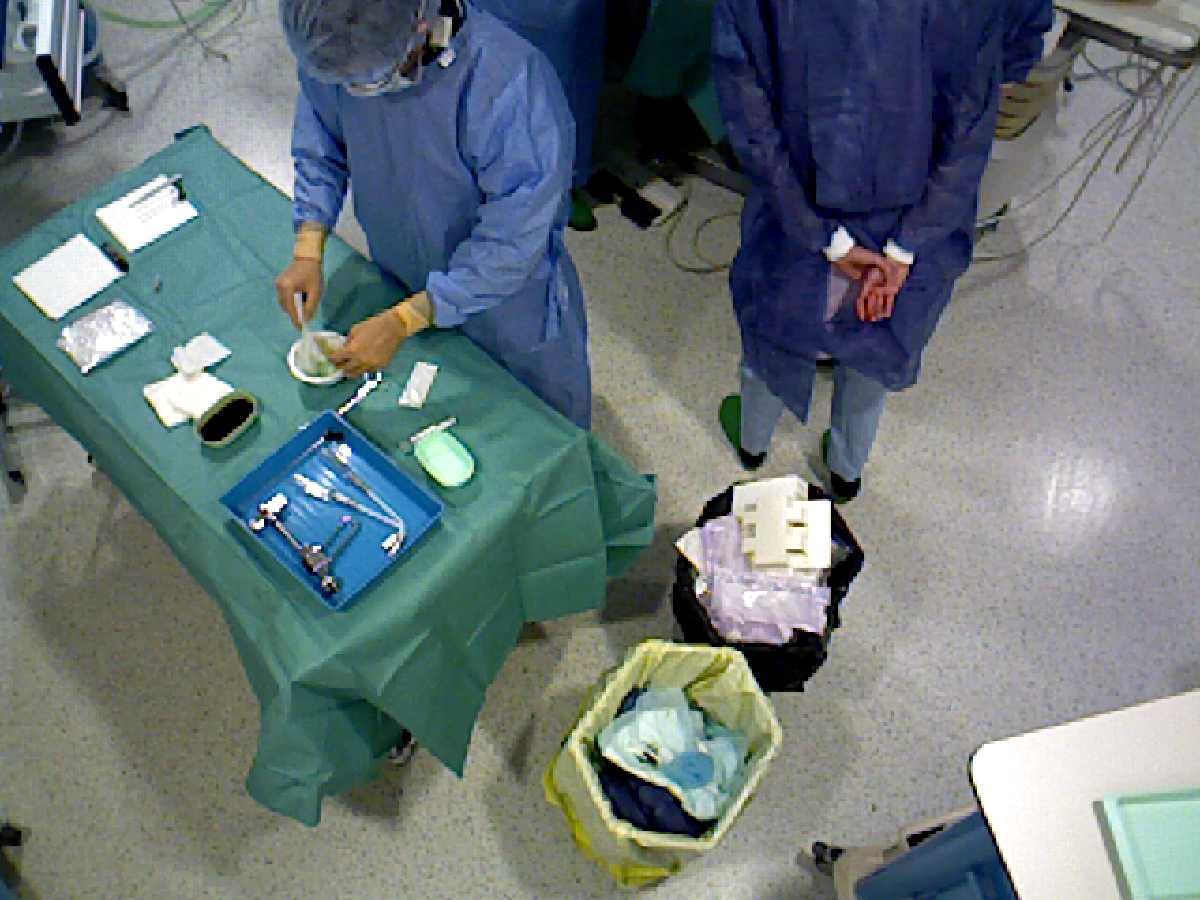
\includegraphics[width=.33\textwidth]{Figures/Actions/13_MixingCement}}\hfill
\subfigure[OpeningPackage]{\label{sfig:n}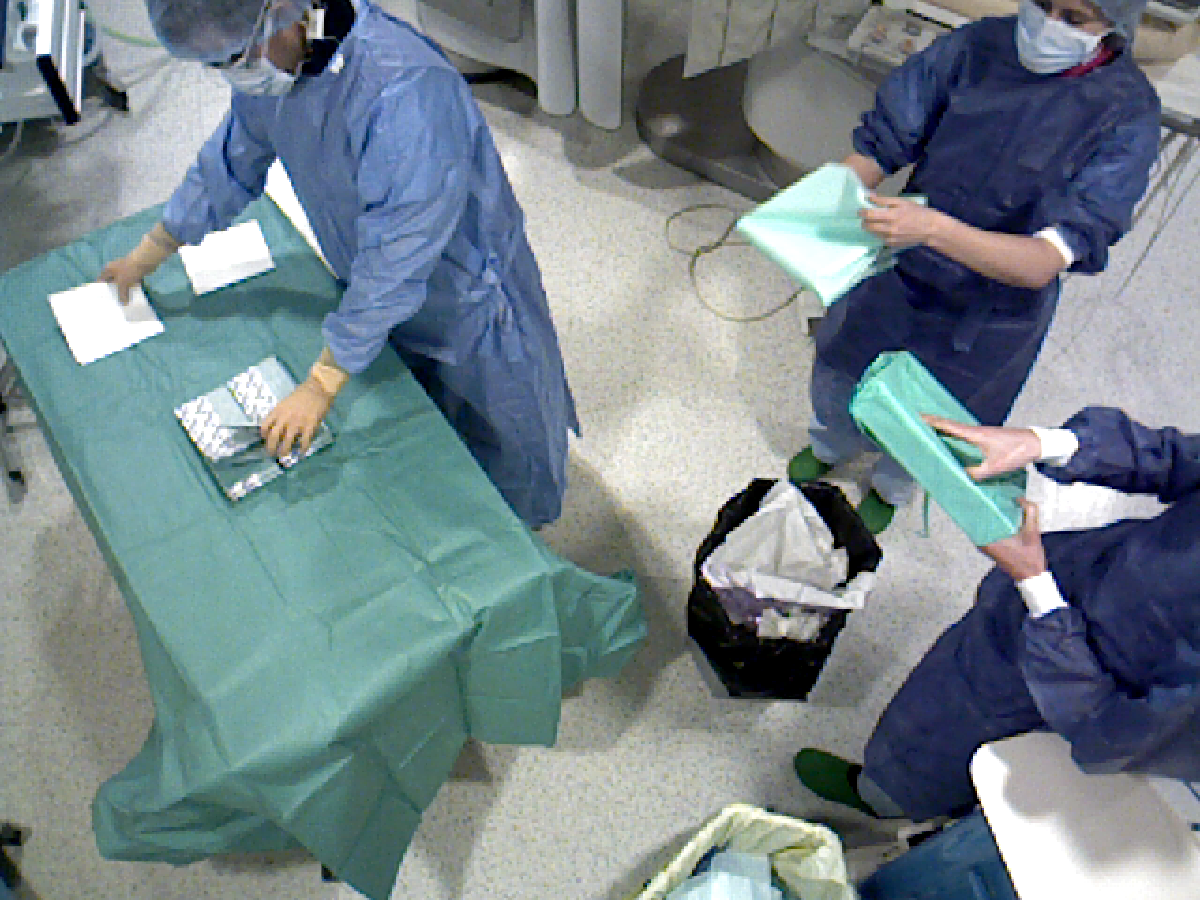
\includegraphics[width=.33\textwidth]{Figures/Actions/14_OpeningPackage}}\hfill
\subfigure[Throwing Package]{\label{sfig:o}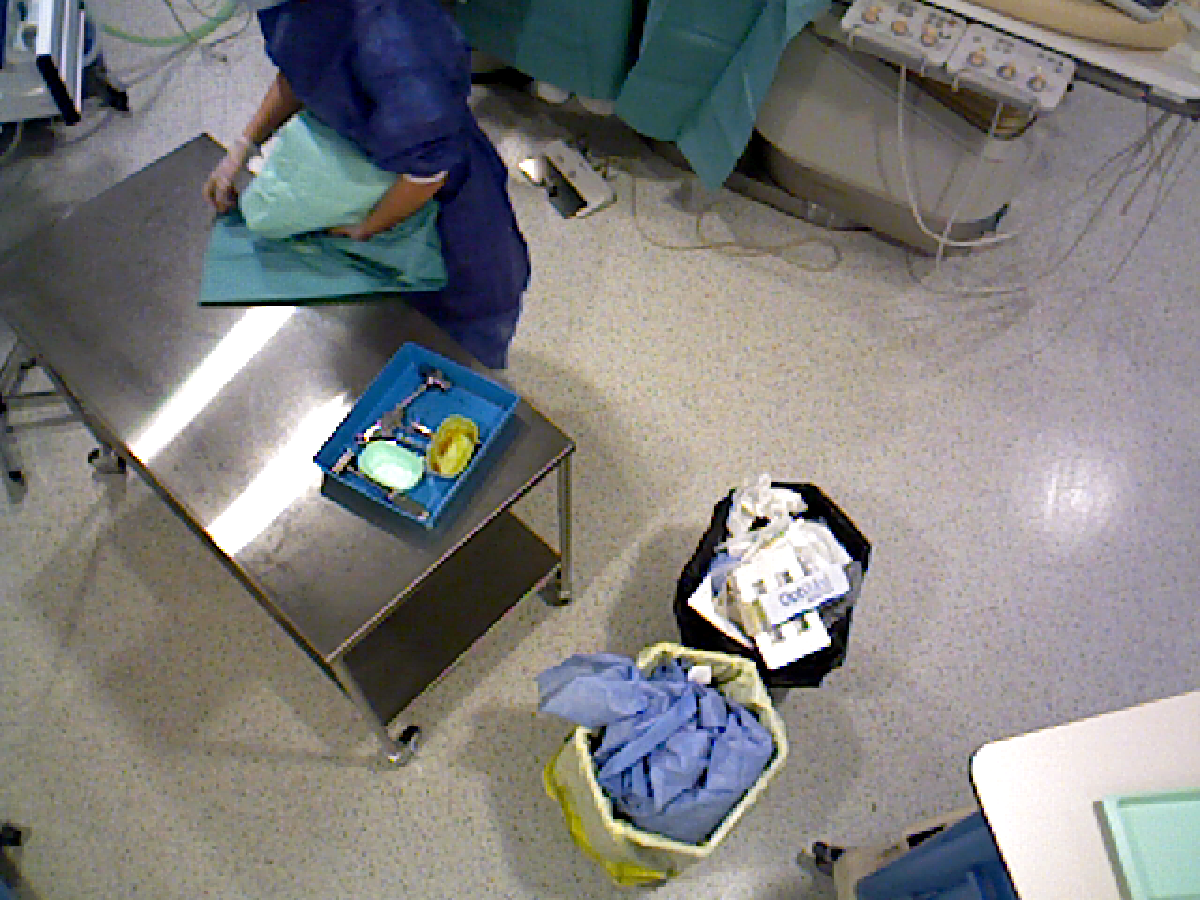
\includegraphics[width=.33\textwidth]{Figures/Actions/15_ThrowingPackage}}\\

\caption{Activity types in the dataset - samples of intensity images}
\label{fig:DatasetActivities}
\end{figure}
    
    	\subsection{Visual feature extraction and encoding}
        \label{section:VisualFeatureExtractionAndEncoding}
        In interest point detection, we detect 1000 STIPs from intensity and 1000 DSTIPs from depth data from each video clip. Then, we extract 480-dimensional HOF from intensity and 4005-dimensional DCSF from depth data around each interest point. We use Principal Component Analysis (PCA) to reduce dimensions of HOF and DSCF to 250 and 800 respectively for visual dictionary construction. All these parameters have proven to produce good results in \citet{twinanda2015data}. In \cite{twinanda2015data}, performance comparison of size of visual dictionaries are studied and it is shown that visual dictionary size 1500 has the highest accuracy and increasing the number of words in dictionary size has not much improve the performance. Then second dictionary, spatio-temporal dictionary, is built to divide 4D spatio-temporal space into non-rigid cells with 24 patches for intensity and depth data. When we use combination of intensity and depth data, the number of 4D patches becomes 48 (24 from both intensity and depth).

        
        \subsection{Classification Setup}
        \label{section:ClassificationStrategy}
        In this work, we use Support Vector Machine (SVM) and Random Forest (RF) classifiers. In the experiments, two-level classification strategy is used and explained in detail in Section~\ref{section:TrainingStrategy}. We also use two different approaches: one-model and multi-model. In one-model approach, a single classifier model is trained on each level. In contrast, in the multi-model approach, multiple classifier models are trained on the first level. For intensity and depth data, 24 classifier models are trained. However, for the combination, 48 classifier models are trained. These numbers are used to match the number of 4D patches.
        
        
        \subsubsection{SVM Setup}
        \label{section:SVMSetup}
         SVM models in the experiments are trained using VLFeat toolbox \cite{Vedaldi:2010:VOP:1873951.1874249}. SVM is used with non-linear kernels, i.e., Chi-square $ \left(\mathcal{X}\right)^{2} $ and histogram intersection kernels. Since there is 15 different classes for classification, one-against-all SVM is used to handle multi-class problem. K-Fold cross validation is used to evaluate performance by dividing the dataset into 10 folds.
        
        \subsubsection{Random Forest Setup}
        \label{section:RandomForestSetup}
        Random Forest models in the experiments are trained using our own implementation of Random Forest. Random Forests depend on many parameters, e.g., number of trees, maximum depth of the trees, minimum information gain and minimum number of samples in each tree node as stopping criteria to stop building a tree. Random Forests are trained with 100 trees, with maximum depth 15. The minimum information gain in the node is set to 0.001 to avoid trees with low information gain. One of the effective parameter in tree building is the minimum number of samples reach to each node before stopping. We use 32 samples as minimum number of samples in node as stopping criteria. Each tree in the random forest have seen 80\% of the training data as randomly for bagging across trees. Finally K-Fold cross validation is used to evaluate the performance by dividing the dataset into 10 folds.


\section{Experimental Results}
\label{section:ExperimentalResults}

In this section, we report results from the voting scheme as well as the comparison with non-voting scheme. We also compare the one-model and multi-model approaches using the proposed two-level classification strategy with the voting scheme, and their results compared on intensity, depth and the combination of the intensity and depth.

%     In this section, we conduct experiments to verify and evaluate our proposed voting scheme strategy on the aforementioned dataset \cite{twinanda2015data} and report the results by comparing to non-voting approach \cite{twinanda2015data}. We use intensity, depth and their combination individually for evaluation using two different classifiers, i.e., non-linear SVM and Random Forest. In the experiments we use two different evaluation methods that changes classification strategy: one-model and multi-model strategies that their setup is described in Section~\ref{ClassificationStrategy}. We share results from the one model and multi model under Section~\ref{section:OneModel} and Section~\ref{section:MultiModel} respectively.
    
\subsection{One Model Approach}
\label{section:OneModelExperiments}
In the one-model approach, we learn a single SVM and Random Forest model in each level with all patches from each activity. In Table~\ref{table:oneModelResults}, results for one-model approach is presented with intensity, depth and combination of the data with both of the classifiers. It is shown that non-linear SVM performs slightly better than the Random Forest. It is also shown that combination of the intensity and depth data has more discriminating power than using only intensity or depth. The combination of the depth and intensity profits the complementary information that intensity and depth carries. Because some activities are well classified in intensity due to illumination and intensity changes, e.g., cement injection, however some actions showed better performance in depth due to high variance in depth, e.g., Adjusting C-Arm. These effects are shown in confusion matrices in Figure~\ref{fig:intensityOneModelConfusionMatrix} and Figure~\ref{fig:depthOneModelConfusionMatrix}. The combination of the intensity and depth data gets the highest accuracy with 83.1\% accuracy using SVM and the confusion matrix is shown in Table~\ref{fig:combinationOneModelConfusionMatrix}.


\begin{table}[h]
\centering
\begin{tabular}{|c|c|c|}
\hline
                     & \textbf{SVM}     & \textbf{RF} \\ \hline
\textbf{Intensity}   & \textbf{74.45\%} & 70.06\%     \\ \hline
\textbf{Depth}       & \textbf{72.72\%} & 67.87\%     \\ \hline
\textbf{Combination} & \textbf{83.1\%}  & 79.18\%     \\ \hline
\end{tabular}
\caption{Classification results using one-model approach}
\label{table:oneModelResults}
\end{table}

\begin{figure}[H]
\begin{center}
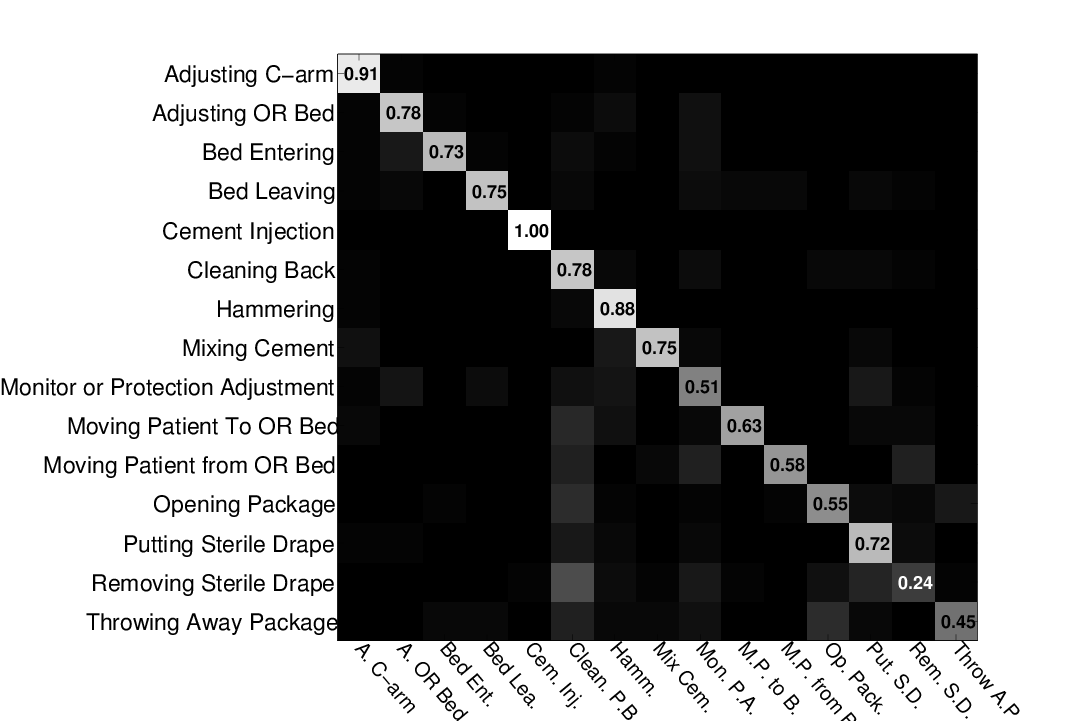
\includegraphics[scale=0.4]{Figures/intensity-onemodel}
\end{center}
\caption{Confusion matrix of one-model approach using intensity features \label{fig:intensityOneModelConfusionMatrix}}
\end{figure}
        
\begin{figure}[H]
\begin{center}
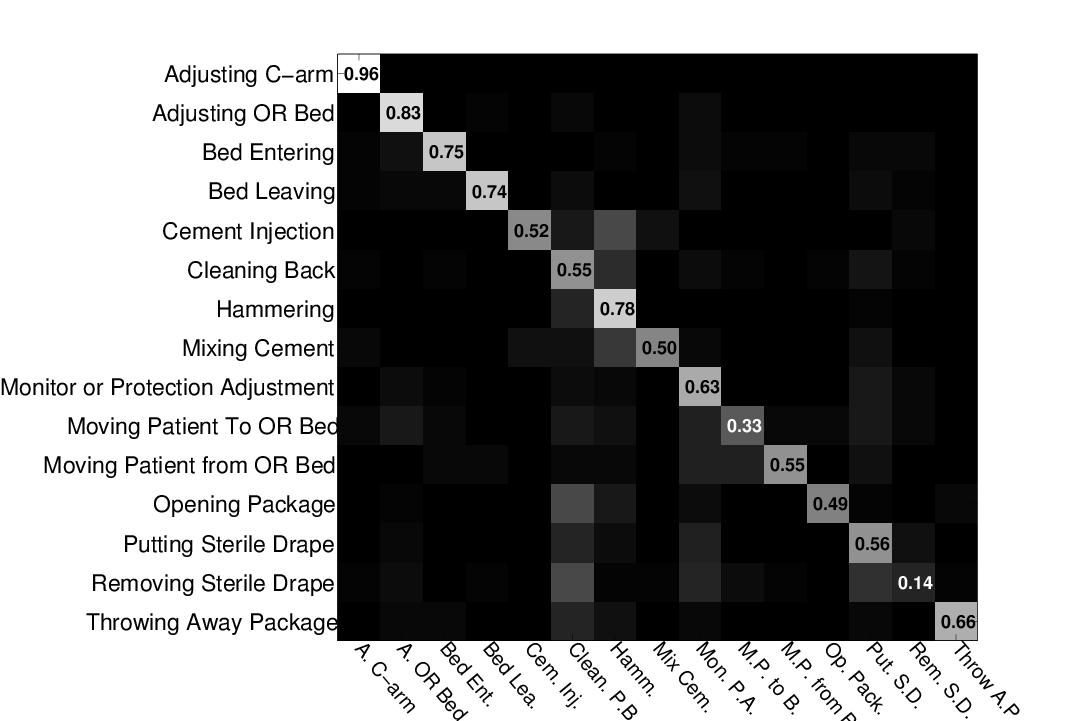
\includegraphics[scale=0.4]{Figures/depth-onemodel}
\end{center}
\caption{Confusion matrix of one-model approach using depth features \label{fig:depthOneModelConfusionMatrix}}
\end{figure}

\begin{figure}[H]%[!htbp]%[here][H]
\begin{center}
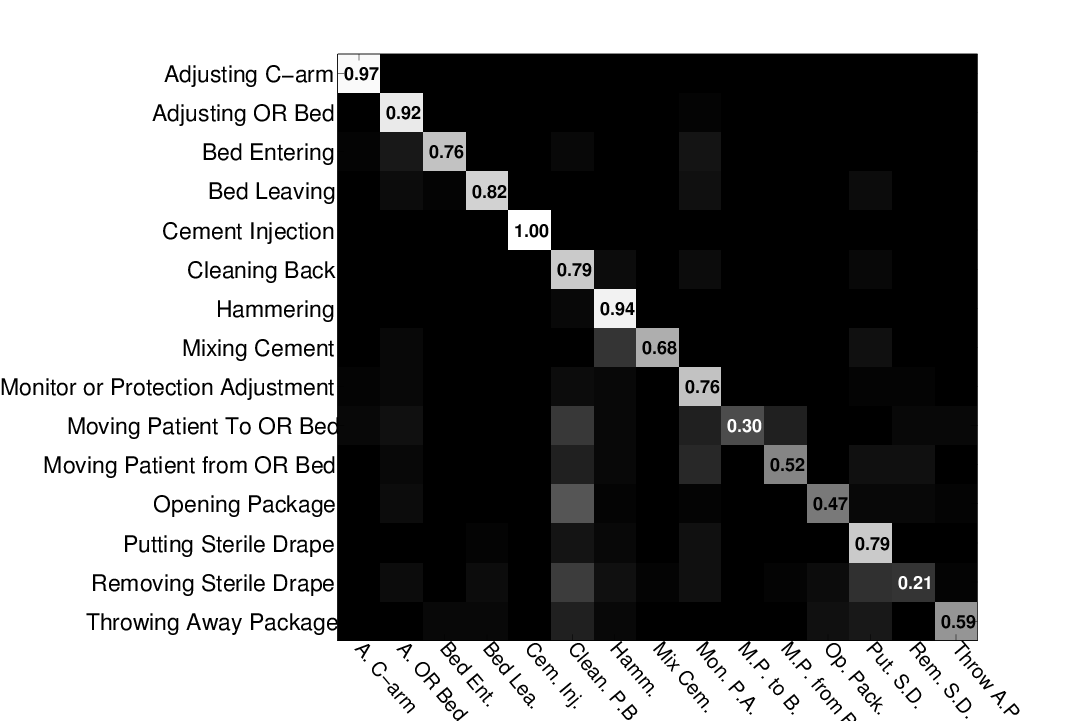
\includegraphics[scale=0.4]{Figures/combination-onemodel}
\end{center}
\caption{Confusion matrix of one-model approach using combination of features
\label{fig:combinationOneModelConfusionMatrix}}
\end{figure}

\subsection{Multi-Model}
\label{section:MultiModelExperiments}
In the multi-model approach, we learn multiple models in the first level for each patch type $P^{j}$. However, the one-model approach in Section~\ref{section:OneModelExperiments} trained a single model for the first level using all the patches from all the video clips.
Hence, one-model approach profits from seeing more training data whereas in the multi-model approach, the first level classifiers sees less training data. Thus, multi-model has slight disadvantage over one-model approach due to training the each patch model. Thus, results presented in Table~\ref{table:multiModelResults} have slighly lesser accuracy than one model results in Table~\ref{table:oneModelResults}. On the other hand, the combination of intensity and depth is still performing better than using only intensity or depth. We achieved 81.71\% accuracy with combination of the data with the SVM classifier. The detailed results are presented with confusion matrices in Figure~\ref{fig:intensityMultiModelConfusionMatrix}, \ref{fig:depthMultiModelConfusionMatrix} and \ref{fig:combinationMultiModelConfusionMatrix}.
            
\begin{table}[H]
\centering
\begin{tabular}{|c|c|c|}
\hline
                     & \textbf{SVM}     & \textbf{RF} \\ \hline
\textbf{Intensity}   & \textbf{77.28\%} & 69.20\%     \\ \hline
\textbf{Depth}       & \textbf{71.91\%} & 64.45\%     \\ \hline
\textbf{Combination} & \textbf{81.71\%} & 75.54\%     \\ \hline
\end{tabular}
\caption{Classification results using multi-model approach}
\label{table:multiModelResults}
\end{table}

\begin{figure}[H]
\begin{center}
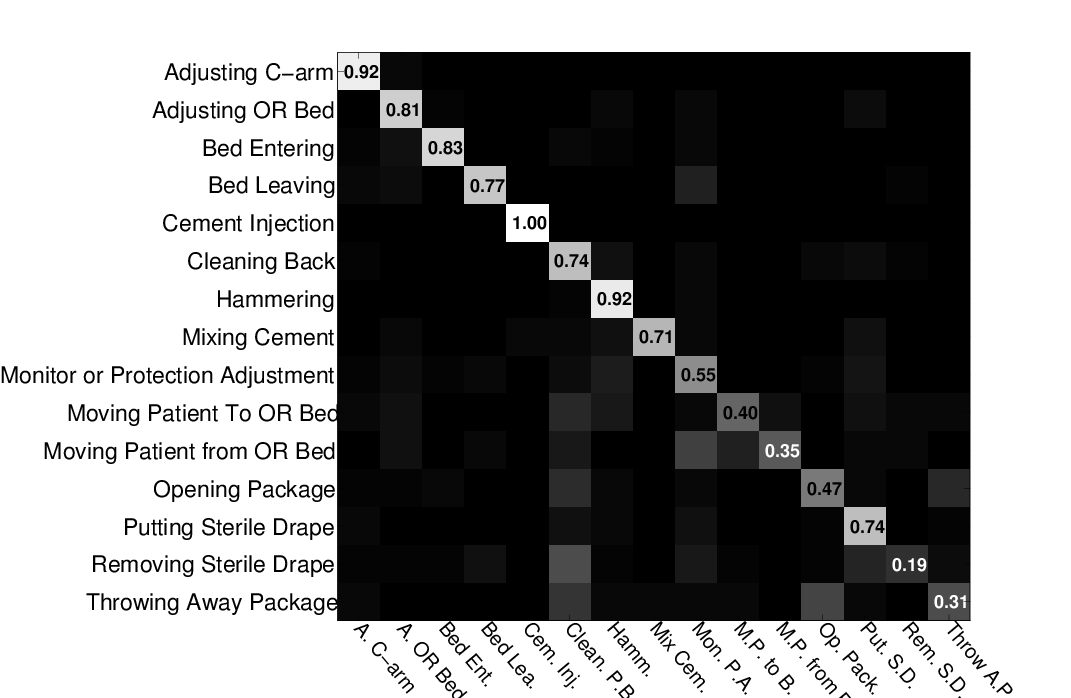
\includegraphics[scale=0.4]{Figures/intensity-multimodel}
\end{center}
\caption{Confusion matrix of multi-model approach using intensity features 
\label{fig:intensityMultiModelConfusionMatrix}}
\end{figure}
        
\begin{figure}[H]
\begin{center}
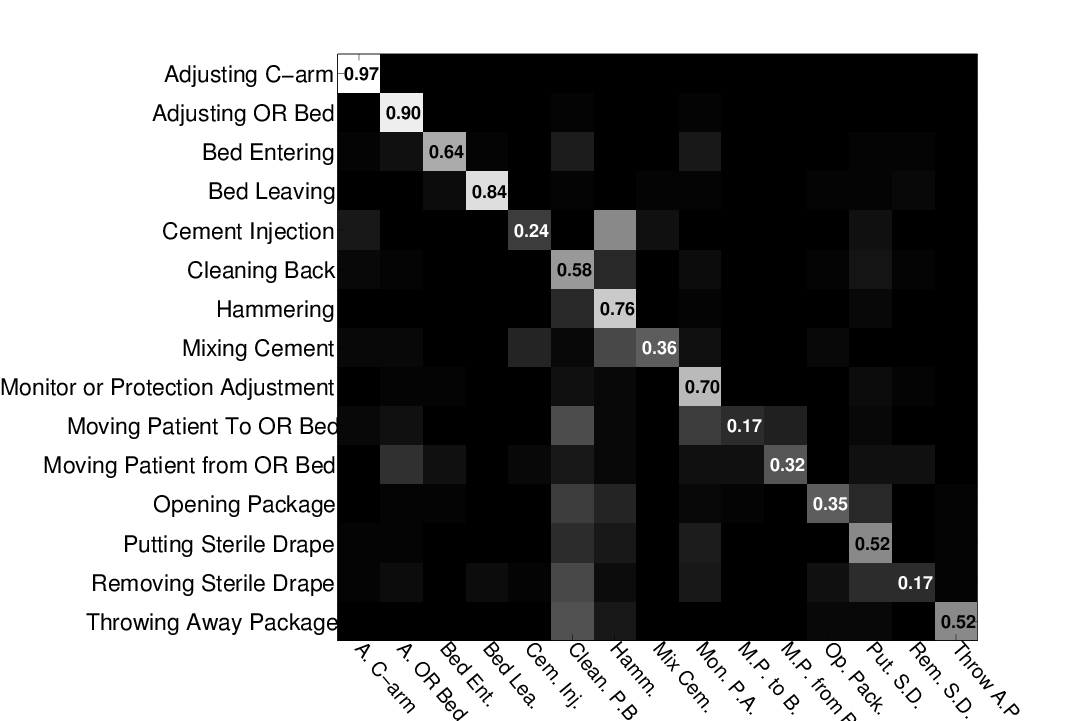
\includegraphics[scale=0.4]{Figures/depth-multimodel}
\end{center}
\caption{Confusion matrix of multi-model approach using depth features  
\label{fig:depthMultiModelConfusionMatrix}}
\end{figure}

\begin{figure}[H]%[!htbp]%[here][H]
\begin{center}
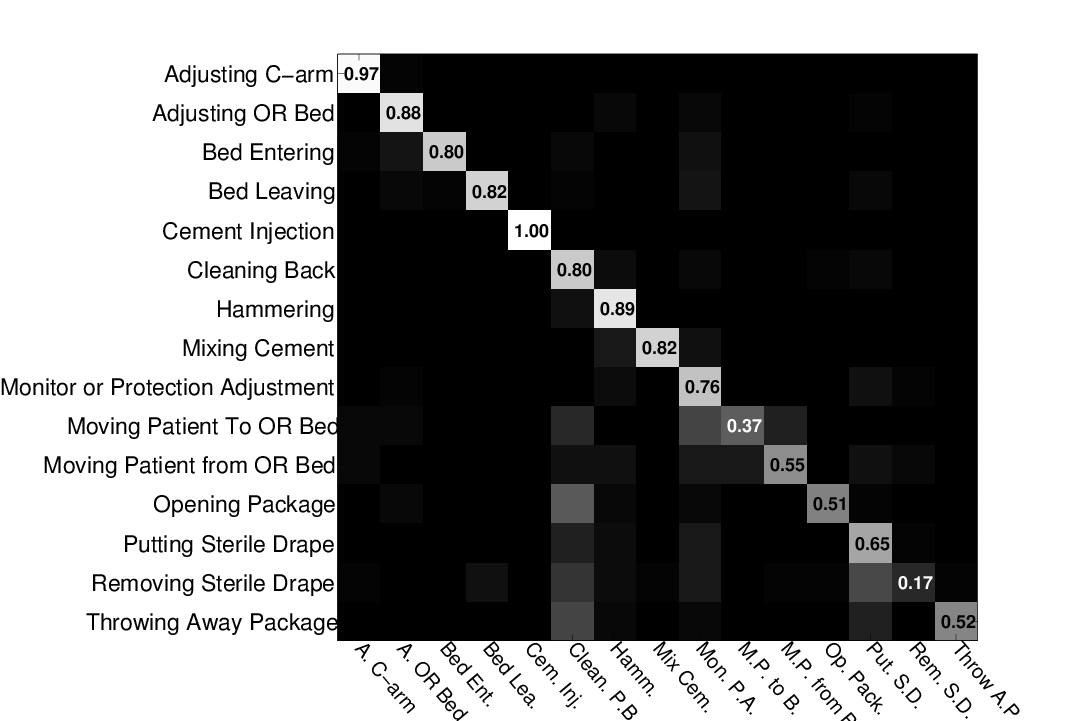
\includegraphics[scale=0.4]{Figures/comb-multimodel}
\end{center}
\caption{Confusion matrix of multi-model approach using combination of features  
\label{fig:combinationMultiModelConfusionMatrix}}
\end{figure}
            
            
            
\subsection{Non-Voting Approach}
\label{section:NonVotingAproachExperiments}
	The proposed voting scheme approach also compared to non-voting scheme approach in \cite{twinanda2015data}. In \cite{twinanda2015data}, a data-driven non-rigid layout is used by concatenating the histogram vectors from patches to construct single histogram vector to represent video clip. The histogram vector also concatenated with a histogram vector extracted from video clip without using any layout. Hence, the final concatenated histogram carries more information than using histograms from each patch separately as in Section~\ref{section:OneModelExperiments} and Section~\ref{section:MultiModelExperiments}. Using the patch histograms separately for training and collecting votes increased the sparsity problem in classification in the first level. The non-voting method reached 85.53\% accuracy compared to our maximum accuracy 83.1\%. The detailed comparison with intensity, depth data and their combination is shown in Table~\ref{table:comparisonResults}.
    
    
\begin{table}[H]
\centering
\begin{tabular}{|c|c|c|}
\hline
                  & {\bf Non-Voting \cite{twinanda2015data}}   & {\bf Voting} \\ \hline
{\bf Intensity}   & {\bf 80.40\%} & 74.45\%    \\ \hline
{\bf Depth}       & {\bf 78.37\%} & 72.72\%    \\ \hline
{\bf Combination} & {\bf 85.53\%} & 83.1\%     \\ \hline
\end{tabular}
\caption{Classification accuracy comparison of non-voting \cite{twinanda2015data} and voting scheme}
\label{table:comparisonResults}
\end{table}
           


\begin{figure}[H]%[!htbp]%[here][H]
\begin{center}
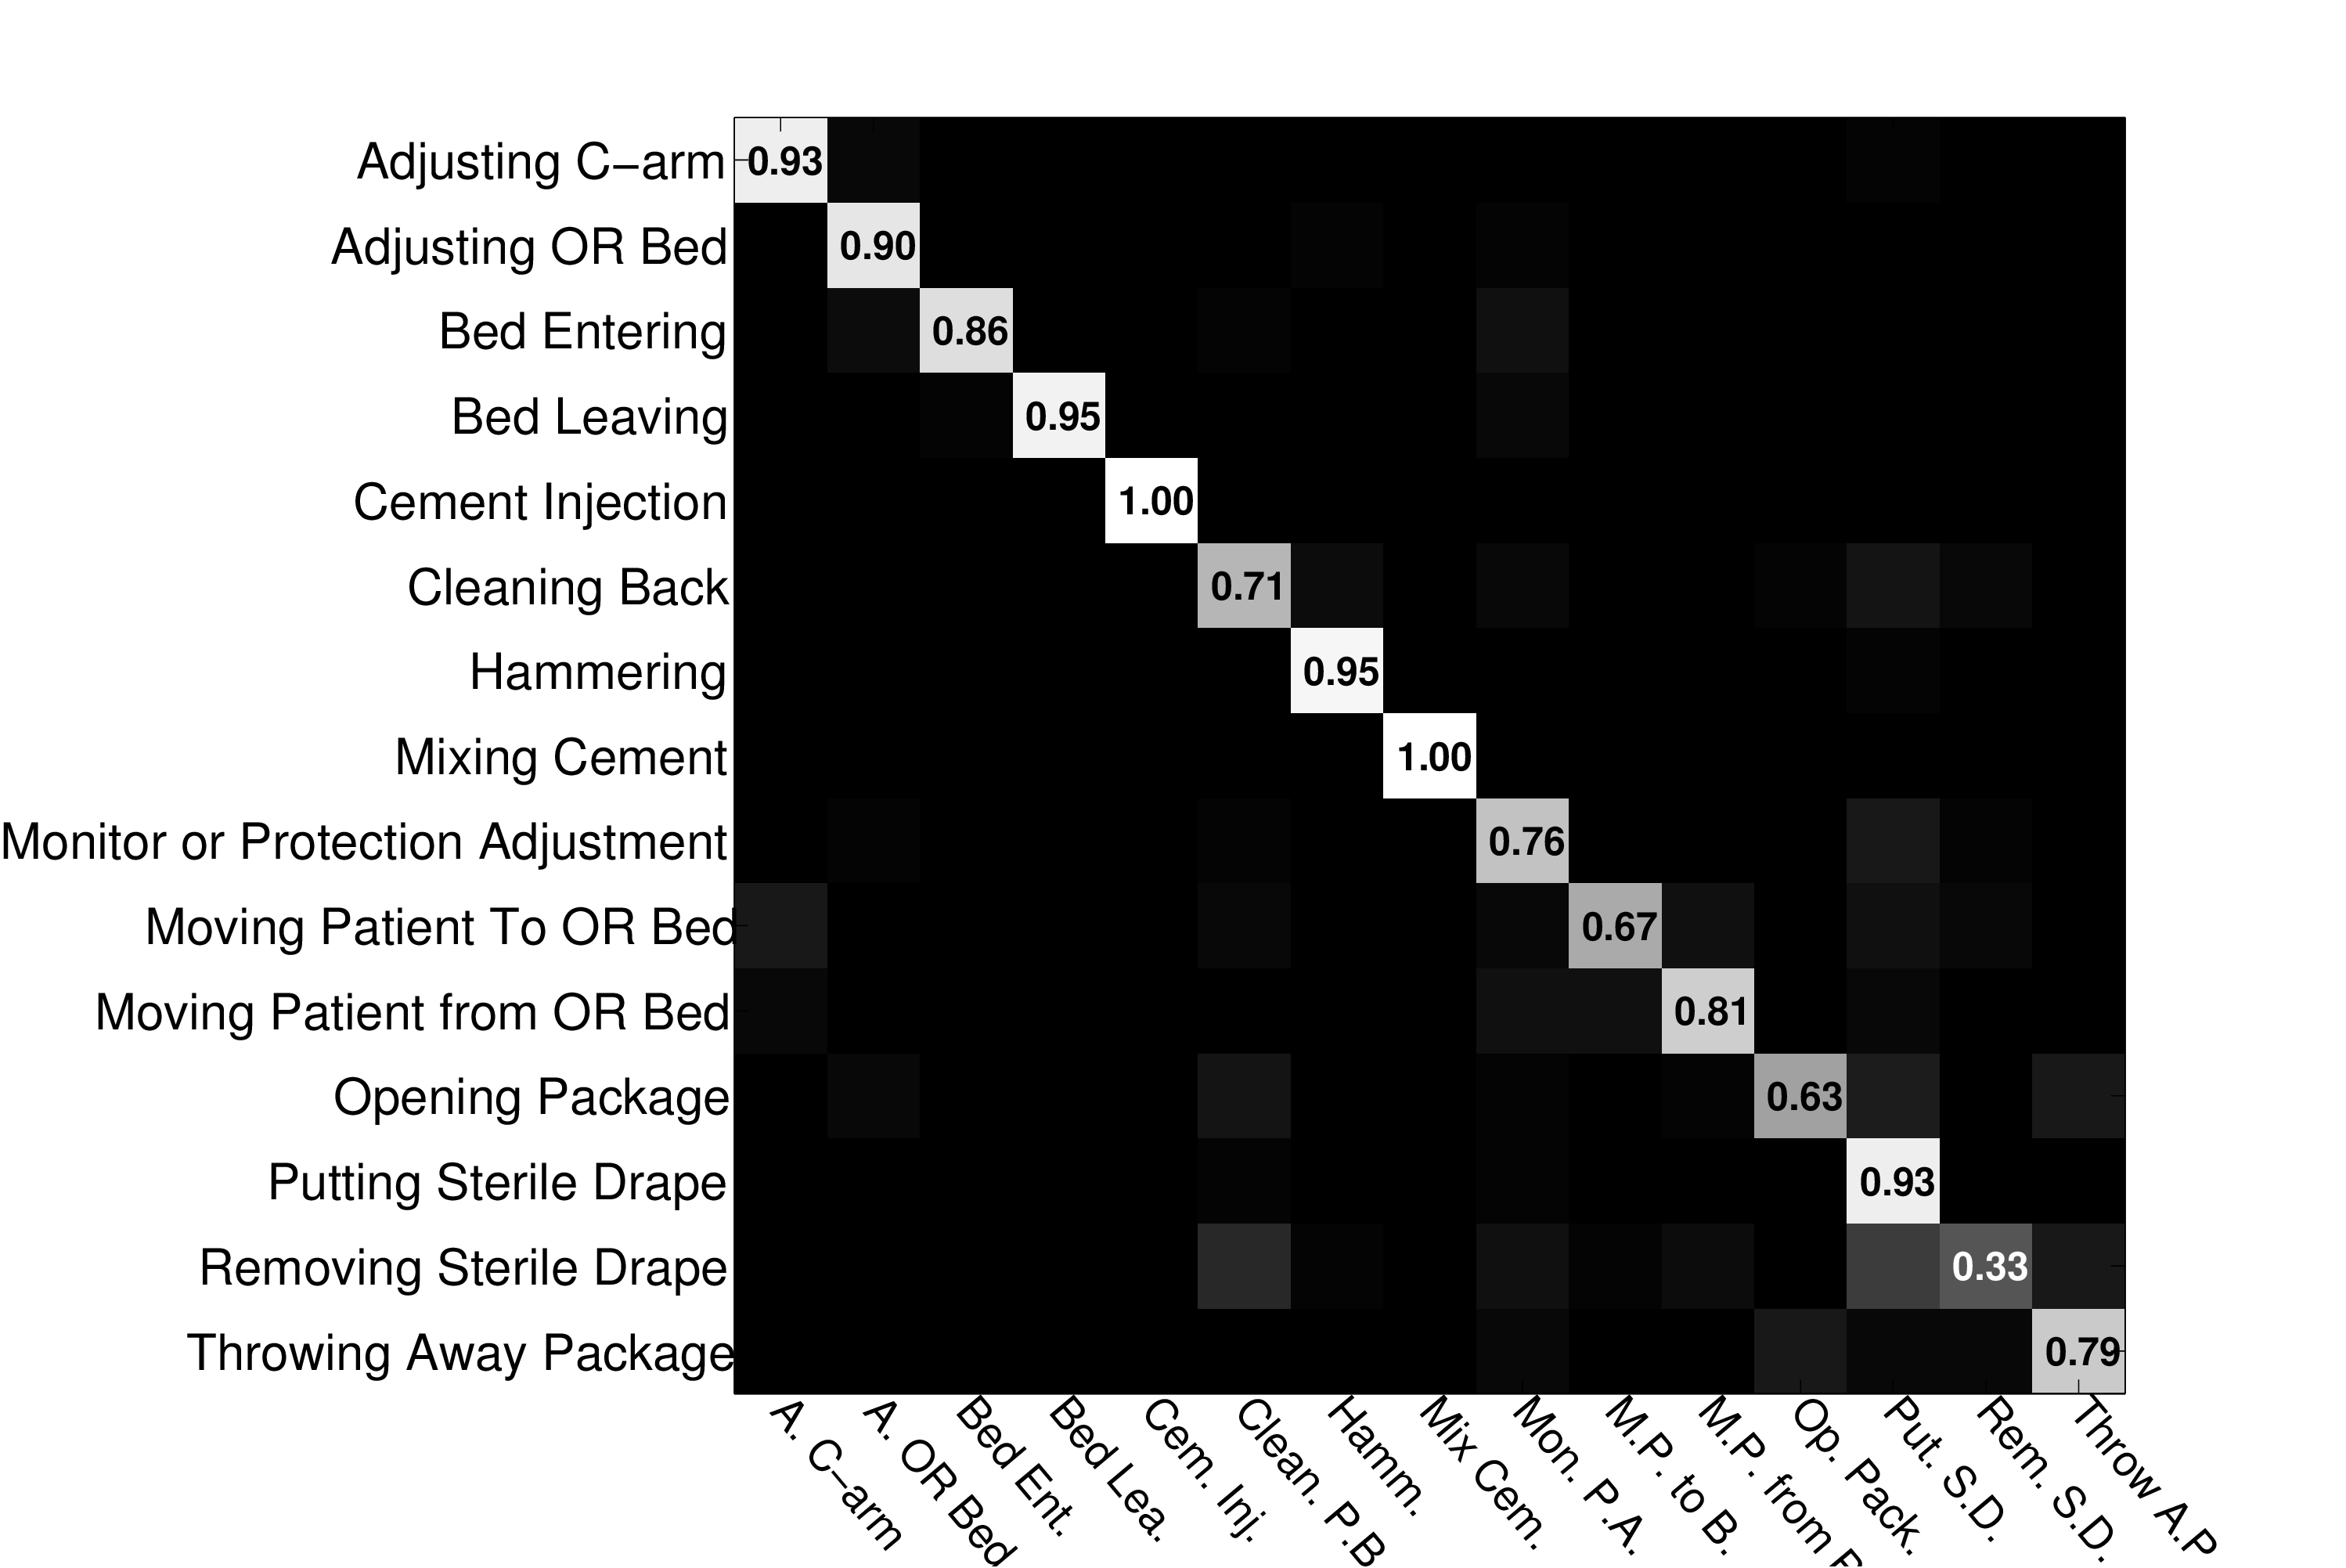
\includegraphics[scale=0.15]{Figures/confusionAndruPaper1}
\end{center}
\caption{Confusion matrix of non-voting scheme using combination of features\cite{twinanda2015data} 
\label{fig:combinationNonVotingConfusionMatrix}}
\end{figure}

In comparison of confusion matrices with voting and non-voting scheme from  Figure~\ref{fig:combinationOneModelConfusionMatrix} and Figure~\ref{fig:combinationNonVotingConfusionMatrix}, it is shown that the voting scheme has better detection on activities, i.e., Adjusting C-Arm, Adjusting OR Bed and Cleaning Back, where in these activities, detected interest points are more separable and informative than other activities. For example, in  Mixing Cement activity, 32\% accuracy decreased in voting scheme approach. In this activity, interest points are detected in very narrow space, and they detected as cluster around the activity, Thus, detected interest points are not uniform in 4D space but distributed around one point. The decrease in the accuracy can be explained as the detected interest points in 4D space is not separated informatively with non-rigid layout for the Mixing Cement activity.



















